\section{Herencia}
\label{herencia}

Como se ha mencionado anteriormente, JavaScript tiene la particularidad de tener la herencia prototipada en vez de la herencia clásica. Este tipo de herencia es bastante poderosa, aunque también a veces incomprendida y mal aplicada.

\subsection{Herencia simple mediante \code{prototype}}

La herencia prototipal es tan potente que, haciendo un esfuerzo y algunos artilugios, se podrá simular la herencia clásica. La diferencia entre estos dos tipos de herencia es que en la herencia clásica, las subclases poseen una copia del comportamiento de clases. En la herencia prototipal no existe este concepto de copia. Un objeto tiene un prototipo y en caso de que el objeto no tenga un atributo o método necesario, delegará esta responsabilidad a su prototipo. Ésto se llama delegación de comportamiento.

Ahora, supongamos el siguiente código:

\begin{lstlisting}[title={Analizando herencia prototipal en JS}]
function Vehiculo(tipo) {
  this.tipo = tipo;
}

Vehiculo.prototype.mostrarTipo = function() {
  console.log(this.tipo);
}

function Auto(marca) {
  Vehiculo.call(this, "terrestre");
  this.marca = marca;
}

Auto.prototype = Object.create(Vehiculo.prototype);
Auto.prototype.constructor = Auto;

Auto.prototype.mostrarMarca = function () {
  console.log(this.marca);
}

var fitito = new Auto("Fiat");
var falcon = new Auto("Ford");
 
fitito.mostrarMarca();      // Fiat
fitito.mostrarTipo();       // terrestre

falcon.mostrarMarca();      // Ford
falcon.mostrarTipo();       // terrestre
\end{lstlisting}

Tal como se mencionó en la sección \ref{clases}, las funciones en JavaScript son un mecanismo por naturaleza para \textit{simular} las clases. ?`Qué sucede en el código de arriba? Se definen las funciones \code{Vehiculo} y \code{Auto} que serán nuestras clases. Ambas funciones actúan de constructoras. Al \code{[[Prototype]]} de \code{Vehiculo} se le agrega un método \code{mostrarTipo} mientras que al \code{[[Prototype]]} de \code{Auto} se le agrega \code{mostrarMarca}. Hasta ese punto es fácil de entender lo sucedido si se ha comprendido las secciones de prototype y de clases. 

?`Qué pasa en las líneas 10, 14 y 15? 
\begin{itemize}
\item Para el caso de la línea 10, la sentencia \code{Vehiculo.call(this, "terrestre")} está simulando una llamada al constructor padre. Lo que sería análogo a hacer \code{super} en Java. Ésta es una de las partes más feas del código, ya que esta llamada debe ser de forma manual, y dándo como parámetro el contexto del invocador.
\item En la línea 14 estamos "`pisando"' el viejo objeto \code{Auto.prototype} que había sido creado al momento de declarar la función \code{Auto}, y creando un nuevo objeto. El método \code{Object.create} crea un nuevo objeto y establece como prototipo del objeto lo que haya sido pasado como primer argumento de la función.
\item La línea 15 es la que quizás muchos programadores suelen omitir. Sin ella, si hacemos \code{console.log(fitito)} o \code{console.log(fitito.constructor)} podemos verificar que nos figura que \code{fitito} es \code{Vehiculo} en vez de \code{Auto}. ?´Por qué sucede esto? En la línea 14, cuando hicimos la vinculación del prototype de \code{Auto} con el prototype de \code{Vehiculo}, creamos un nuevo objeto y hemos perdido la referencia de \code{Auto.prototype.constructor}.
\end{itemize}

En ejecución, podemos imaginarnos la siguiente imagen como una representación de lo que hay en memoria:

\newpage

\begin{figure}[H]
\centering
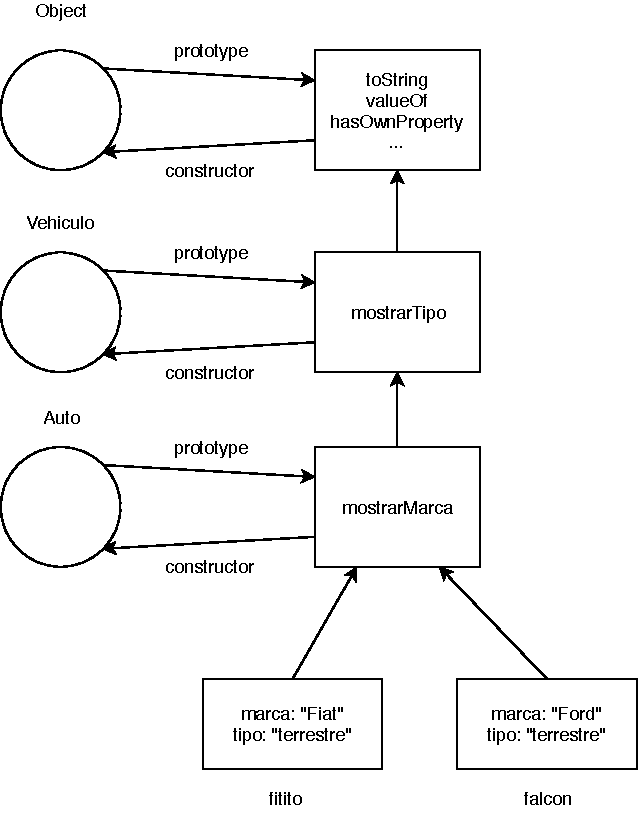
\includegraphics{Figures/Herencia}
\decoRule
\caption[Herencia prototipada]{Diagrama del código presentado}
\label{fig:herencia}
\end{figure}

\subsection{\code{extends} en ES6}

Tal como se explicó sobre la palabra reservada \code{class} en la sección \ref{clasesenes6}, otra de las características que se introdujeron a partir de la versión ES6 es la de la palabra \code{extends} para simular la herencia de clases. Análogo a lo que ocurría con \code{class}, ésta característica es meramente \textit{syntactic sugar} que le omite al programador la necesidad de pensar en prototipos. 

\begin{lstlisting}[title={\code{extends} en ES6}]
class Vehiculo {
  constructor(tipo) {
    this.tipo = tipo;
  }
  mostrarTipo() {
    console.log(this.tipo);
  }
}

class Auto extends Vehiculo {
  constructor(marca) {
    super("terrestre");
    this.marca = marca;
  }
  mostrarMarca() {
    console.log(this.marca);
  }
}

var fitito = new Auto("Fiat");
var falcon = new Auto("Ford");
     
fitito.mostrarMarca();      // Fiat
fitito.mostrarTipo();       // terrestre

falcon.mostrarMarca();      // Ford
falcon.mostrarTipo();       // terrestre
\end{lstlisting}

Para el programador que viene de C++ o Java, este uso de \code{class} y \code{extends} es, por lejos, muchísimo más amigable que crear funciones y vincularlas mediante sus prototipos. Otra de las introducciones a partir de ES6 es el uso del \code{super} en el constructor. Esto facilita enormemente la llamada al constructor de la superclase, o de métodos de la superclase, además de mimetizar la sintaxis de Java. 

\subsection{Herencia múltiple}

Dado que los objetos "`heredan"' de un único prototipo, el lenguaje no provee ninguna herramienta natural para el soporte de la herencia múltiple. Otros lenguajes buscan alcanzar la herencia múltiple mediante el uso de interfaces. En JavaScript no existen las interfaces, pero sí existe una técnica llamada mixins (acrónimo para \textit{mixed in}, del inglés "`mezclado"') para introducir un comportamiento a una clase sin necesidad de hacerla heredar de otra.

Una función de Mixin suele tener esta forma:

\begin{lstlisting}[title={Función de Mixin}]
function mixin(fuente, destino) {  
  for (var prop in fuente) {
    if (fuente.hasOwnProperty(prop)) {
      destino[prop] = fuente[prop];
    }
  }
}
\end{lstlisting}

Lo ideal sería pensar en \code{fuente} como un objeto cuyas propiedades serán los miembros a "`inyectar"' en \code{destino}. Esta técnica llevó al estándar a agregar un método \code{Object.assign} a partir de ES6, el cual copia los valores de todas las propiedades enumerables en un objeto destino.

Otra manera de implementar los Mixins en ES6 es aprovechando que las clases son de primer órden. Éstas pueden ser pasadas como argumento o ser retornadas por una función.

\begin{lstlisting}[title={Haciendo uso de \code{class} como expresión}]
var MyMixin = (superclass) => class extends superclass {  
  saludar() {
    console.log("hola!");
  }
};

class Foo {}
class Bar extends MyMixin(Foo) {
  despedirse() {
    console.log("chau!");
  }
}

var objeto = new Bar();

objeto.saludar();			// hola!
objeto.despedirse();	// chau!
\end{lstlisting}

Como se puede observar, existen varias formas de aplicar esta técnica. Como se mencionó anteriormente, no hay soporte para herencia múltiple en JavaScript, aunque ésta es una forma de resolver el problema. Aún así, tiene sus defectos. El \textit{shadowing} u \textit{overriding} de métodos con el mismo identificador es una convención a tener en cuenta. También hay que pensar en el costo, ya que copiar las propiedades de un objeto a otro requiere de un esfuerzo.
